\FloatBarrier
\section{Communication with Heicub}
\label{sec::34_co}
With YARP \cite{metta2006yarp}, it is possible to directly interface the robot's motors, the cameras, and the force torque sensors. Moreover, it enables the user to run multiple programs in parallel, which can then communicate with each other, which is of special importance for the control loop that was implemented within the scope of this thesis (see figure \ref{fig::3_yarp}).
\begin{figure}[h!]
	\centering
	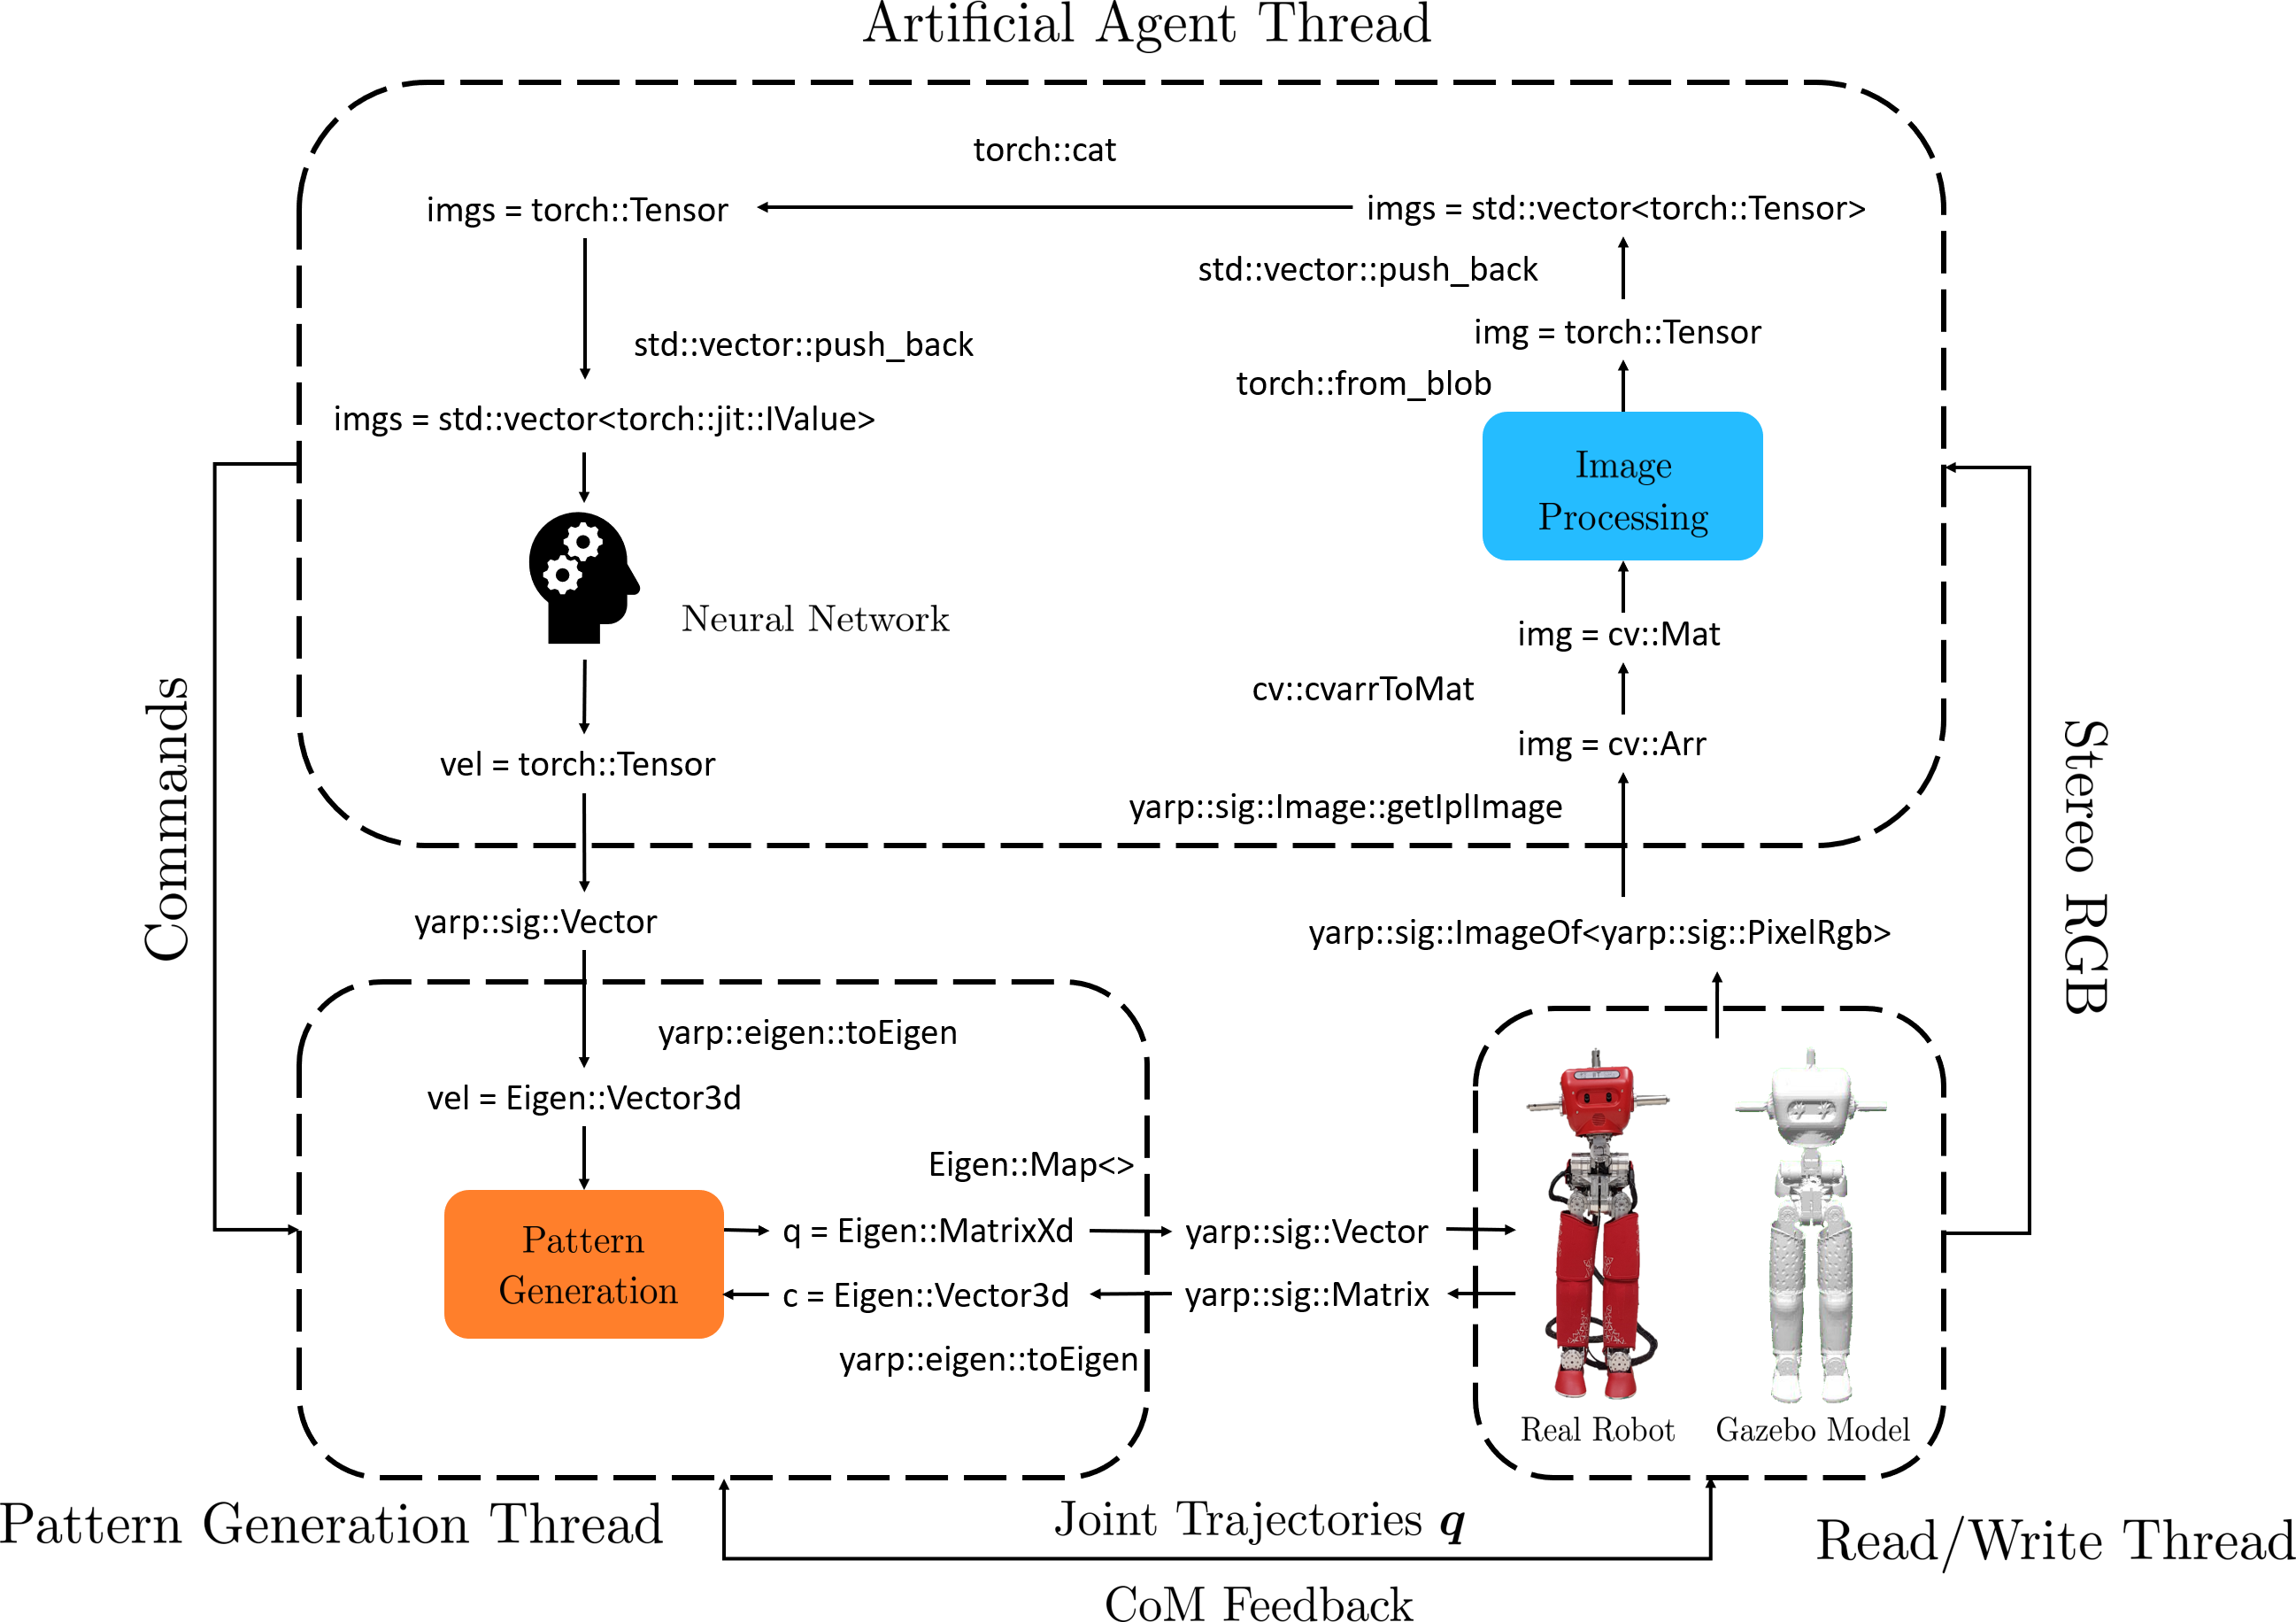
\includegraphics[scale=.4]{chapters/03_methods/img/yarp_diag.png}
	\caption{YARP is used to run multiple threads in parallel, each of which is indicated by the dashed boxes. It further enables the individual threads to communicate with each other via ports. It enables communication to the real robot as well as to a simulated version of it. Notice that this is an extended version of figure \ref{fig::2_cl}.}
	\label{fig::3_yarp}
\end{figure}
As we know from the previous section, one of these threads is committed to take decisions with a neural network, given RGBD images. This thread is depicted as the artificial agent thread in figure \ref{fig::3_yarp}. The pattern generation thread performs the nonlinear model predictive control, given the velocity command of the artificial agent thread. Furthermore, there are two additional threads running that communicate with Heicub's motors. These threads are the read, and the write thread in figure \ref{fig::3_yarp}. The classes, which implement the communication to the robot, are located within the io\_module folder of figure \ref{sec::A_si}. The \inlinecode{C++}{WriteJoints} class implements a \inlinecode{C++}{yarp::os::RateThread}, which is periodically being called, to accesses the motors, which are defined within the YAML configuration file, and changes the motors' settings to position direct mode. Therefore, whatever is being written to the port that \inlinecode{C++}{WriteJoints} uses to communicate with the YARP network, and which is defined in the YAML configuration file, directly gets executed on the robot's motors. This communication to Heicub's motors corresponds to the very lowest part of figure \ref{fig::3_yarp}, where, as extensively explain in section \ref{sec::32_pg}, the pattern generation uses the forward kinematics to generate joint angles $\bm{q}$, which are being written as \inlinecode{C++}{yarp::sig::Vector} to the \inlinecode{C++}{WriteJoints} rate thread. The reading of the robot's sensors is also implemented as part of the io\_module folder in figure \ref{fig::31_folder}. There are several classes, which implement \inlinecode{C++}{yarp::os::RateThreads} for different tasks. Among them are the \inlinecode{C++}{ReadJoints} class, which reads out the motor encoders to obtain the joint angles, the \inlinecode{C++}{ReadCameras} class, which reads out the cameras and pushes them as \inlinecode{C++}{yarp::sig::ImageOf<yarp::sig::PixelRgb>} onto the network (see figure \ref{fig::3_yarp}), the \inlinecode{C++}{AppReader} class, and the \inlinecode{C++}{KeyReader} class, which handle the communication to the joystick app, and the terminal, respectively. Both, the \inlinecode{C++}{AppReader} class, and the \inlinecode{C++}{KeyReader} class, utilize NCurses to generate a user interface on the terminal, which is internally being trapped in a while loop until exit. They readout the input, which may originate from the joystick app, or the keyboard, and push them as the velocity commands onto the YARP network (see figure \ref{fig::3_yarp} left). The velocity commands, which are converted into an \inlinecode{C++}{Eigen::Vector3d} for the \inlinecode{C++}{NMPCGenerator::SetVelocityReference} method from section \ref{sec::32_pg}, may alternatively also originate from a neural network, which is being presented in figure \ref{fig::3_yarp}. The \inlinecode{C++}{GenerateVelocityCommands} rate thread, which enables this feature, is implemented as part of the src folder in \ref{fig::31_folder}, as it only utilizes the provided libraries. It can be found at the provided \href{https://github.com/mhubii/nmpc_pattern_generator/blob/719fde0bb73925923de85cbf379c5523e075dfeb/src/behavioural_augmentation_real_robot_external_data.cpp#L108}{\underline{link}}. Its main task is to read in the images, which are constantly being pushed to the YARP network by \inlinecode{C++}{ReadCameras}, and to convert them into \inlinecode{C++}{cv::Mat} matrices, for us to perform the image processing on them, which includes the rectification, and the depth map extraction that are explained in section \ref{sec::224_ip}. The \inlinecode{C++}{GenerateVelocityCommands} class additionally stores a sequence of the processed images in the form of a \inlinecode{C++}{std::vector<torch::Tensor>}. Whenever a new image is read from the YARP network, the oldest image within the \inlinecode{C++}{std::vector<torch::Tensor>} is being deleted, and all other images are shifted up by one index, such that the newest image is available as the first entry. This vector of tensors is then being converted into a single tensor, by concatenating the individual tensors along the first dimension, which is by definition of the long short term memory units required in PyTorch. The concatenated tensor is further being converted into a \inlinecode{C++}{std::vector<torch::jit::IValue>}, such that the JIT script, which defines the neural network that got trained in Python (see \ref{sec::33_dl}), can forward it. The output is then obtained as a \inlinecode{C++}{torch::Tensor} yet again, which is being written in the form of a \inlinecode{C++}{yarp::sig::Vector} to the YARP network, such that,  as explained above, the pattern generation can use it as input. This pipeline works equivalently on the real robot, as well as on a simulated version of it in Gazebo \cite{koenig2004design}, for which install instructions are provided in the appendix \ref{sec::A4_sm}. It therefore allowed us to prototype within the simulation, yet, as example for our method, we will use the pipeline to train Heicub on finding a fire extinguisher within the next section - Experiments.

